\subsection{Red Subte D}

Para el último experimento, capturamos los paquetes de la LAN Wi-Fi Subte-BA de la estación Plaza Italia de la Línea D del Subte de Buenos Aires.La medición fue realizada un día Domingo a las 16.30hs y durante solamente 1 minuto (por motivos externos). Capturamos 1.000 paquetes de los cuales 25 son ARP.

\begin{figure}[H]
       \centering
       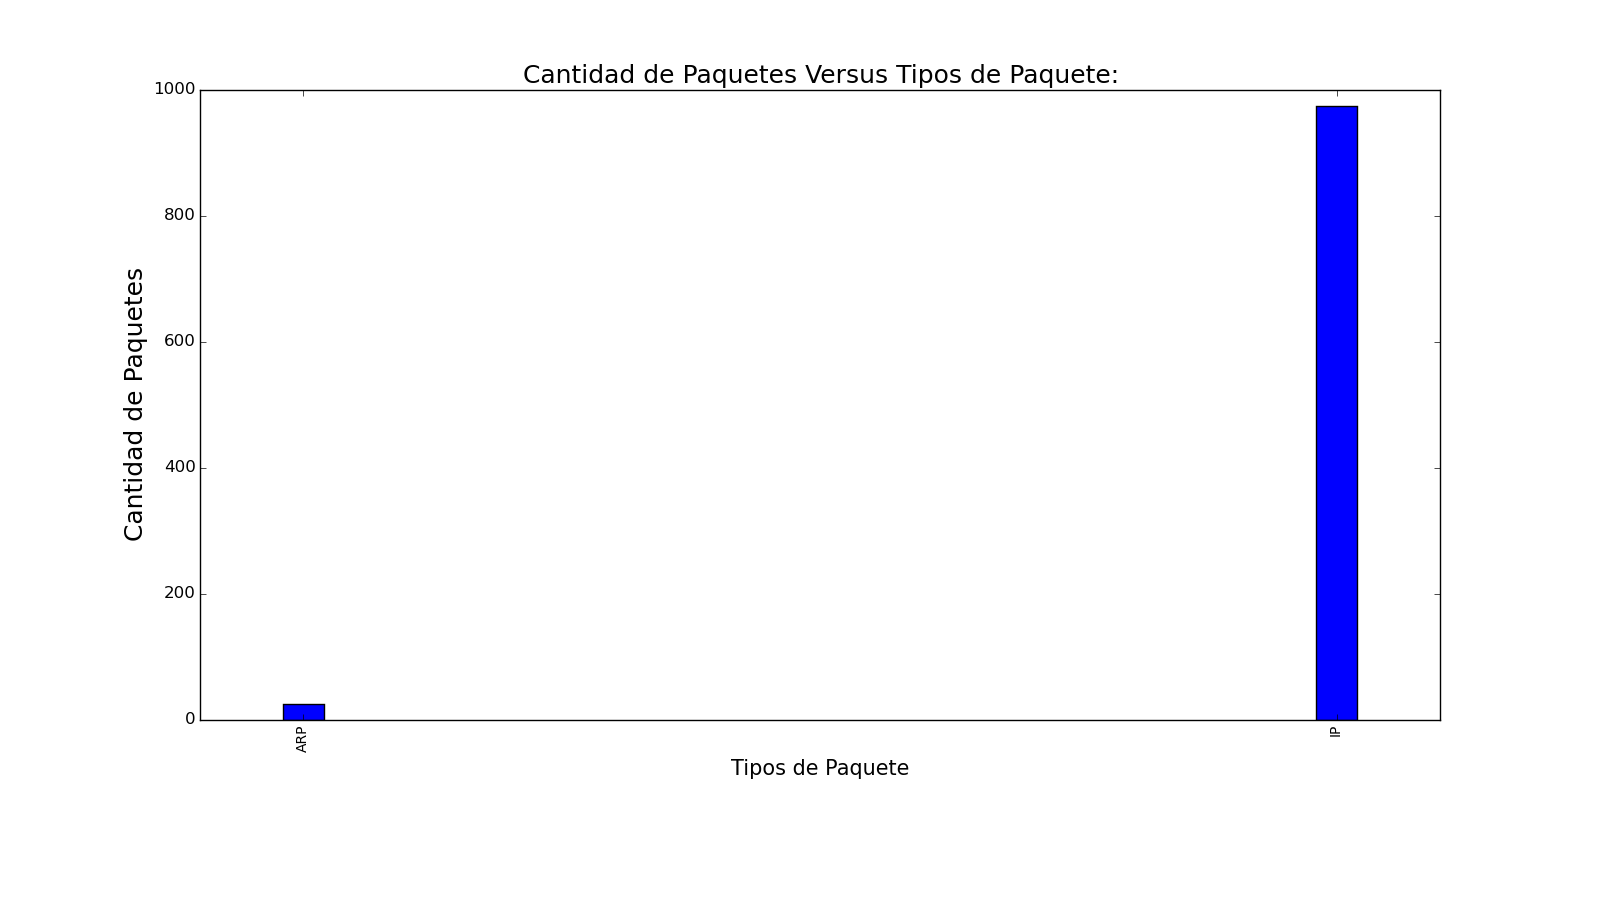
\includegraphics[width=1\textwidth]{../resultados/subte/histogram_types.png}
       \caption{Protocolos de los paquetes capturados}
       \label{red-Starbucks-types}
\end{figure}

En este caso, el overhead impuesto por los paquetes ARP es de 2.5\%.

\begin{figure}[H]
       \centering
       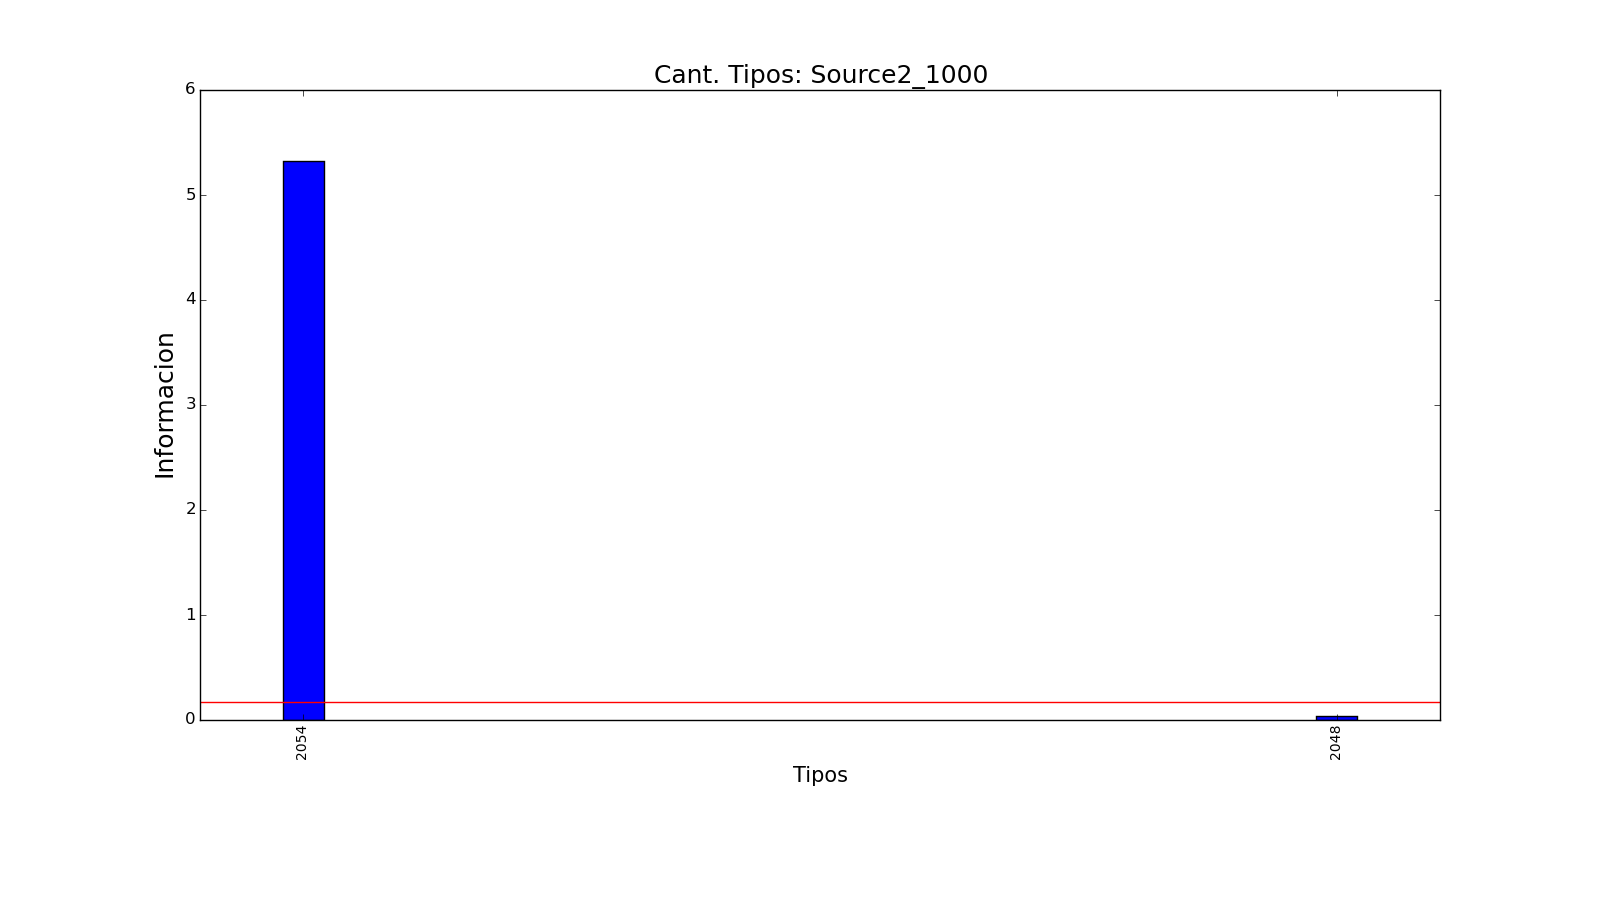
\includegraphics[width=1\textwidth]{../resultados/subte/histogram_types_information.png}
       \caption{Información de los protocolos de los paquetes capturados}
       \label{red-Starbucks-types-information}
\end{figure}

Como podemos también en este experimento, el protocolo IPv4 sería el único distinguido en esta fuente. Es razonable, ya que la cantidad de paquetes IPv4 es mucho mayor que la cantidad de paquetes ARP. La información de los paquetes IPv4 es \textbf{5.32192809489}, mientras que la entropía de la fuente es \textbf{0.168660931497}. Se observa como la información es muy menor a la entropía.

\begin{figure}[H]
       \centering
       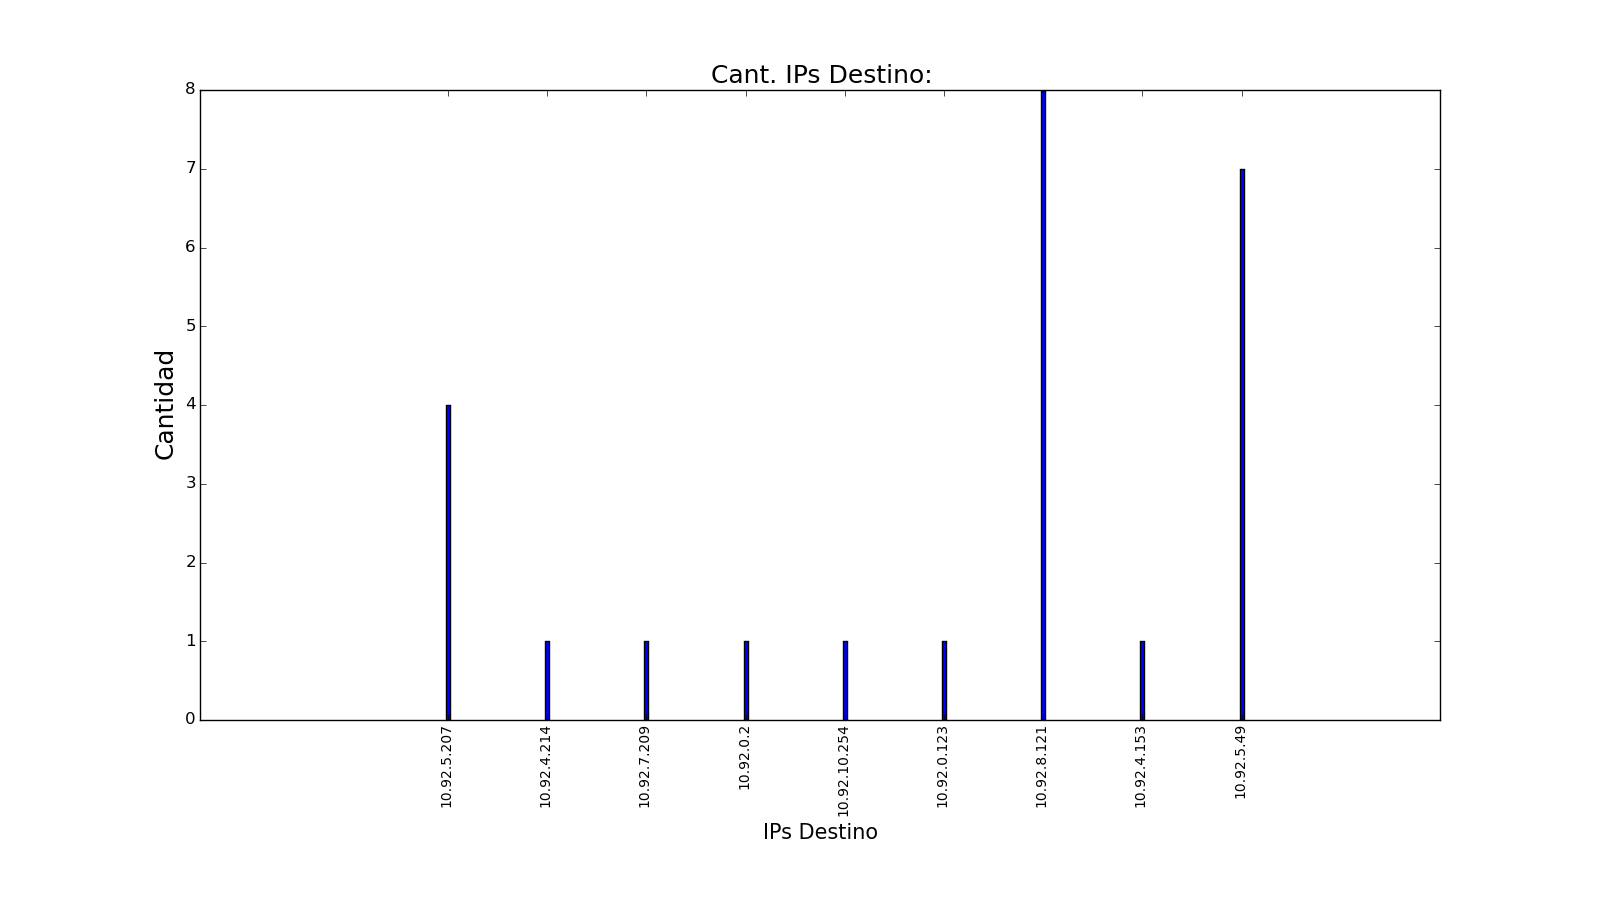
\includegraphics[width=1\textwidth]{../resultados/subte/histogram_dst.png}
       \caption{IPs destino de los paquetes ARP}
       \label{red-Starbucks-dst}
\end{figure}

\begin{figure}[H]
       \centering
       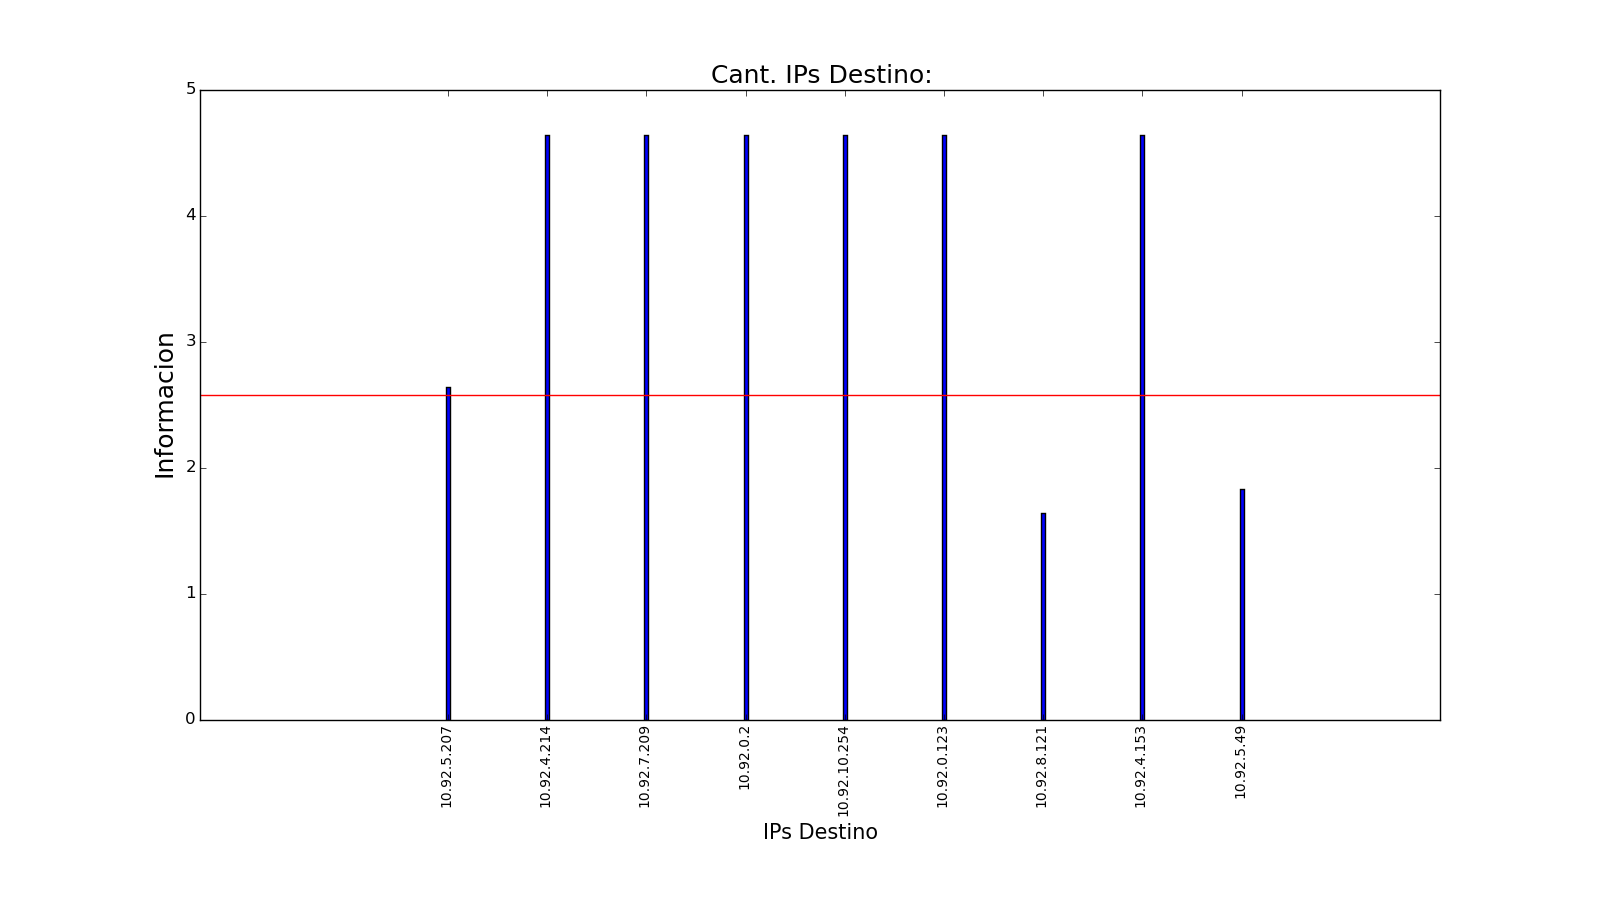
\includegraphics[width=1\textwidth]{../resultados/subte/histogram_dst_information.png}
       \caption{Información de IPs destino de los paquetes ARP}
       \label{red-Starbucks-dst-information}
\end{figure}

\begin{figure}[H]
       \centering
       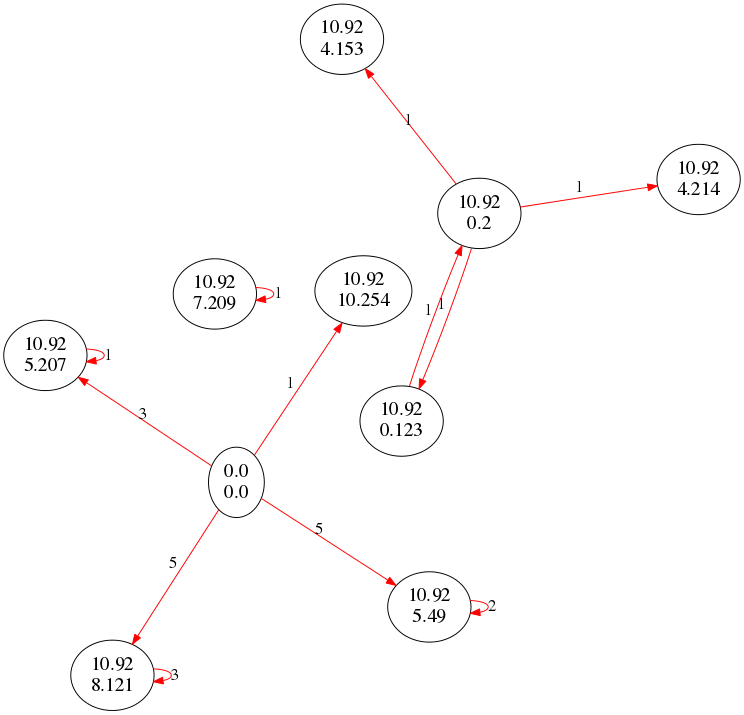
\includegraphics[width=1\textwidth]{../resultados/subte/network.png}
       \caption{Tráfico de paquetes ARP}
       \label{red-Starbucks-dst-information}
\end{figure}

Analizando los gráficos podemos ver que las IPs \textbf{10.92.8.121} y \textbf{10.92.5.49} reciben una mayor cantidad de paquetes que las demás y son nodos distinguidos por ser su información menor a la entropía. Pero los paquetes que reciben tienen como origen a la IP \textbf{0.0.0.0}, que como discutimos en la siguiente sección, son ARP requests que se mandan debido a la ejecución de un protocolo DHCP. No podemos sacar más conclusiones de estos gráficos debido al corto tiempo de intercepción de paquetes.\\
